% !TeX root = skripta-konstitutivni-vztahy-materialu.tex
% !TeX lastmodified = 2019-11-20

\subsection{Model Ogden-Roxburgh}\label{sec:ogden-roxburgh}
Tento pseudoelastický model\footnote{Ogden RW, Roxburgh DG (1999): A pseudo-elastic model for the Mullins effect in filled rubber. Proc. Royal Society London A, Vol. 455, pp. 2861-2877.} byl navržen v~roce 1999 pro popis Mullinsova efektu, který je významný zvláště u~plněných elastomerů.
Model sestává z~funkce měrné energie napjatosti $\psi_0$ pro popis panenské materiálové křivky, která se modifikuje při odlehčovacím a~dalších zatěžovacích cyklech korekčním faktorem (damage parameter) $\eta$, snižujícím úroveň napětí v~závislosti na předcházející maximální hodnotě zatížení $\psi_0^\text{max}$:
\begin{align}
	\psi(\bm{F}, \eta) &= \eta \psi_0(\bm{F}) + \varPhi(\eta),\\
	\eta &= 1 - \frac{1}{r} \mathrm{erf}\left( \frac{\psi_0^\text{max} - \psi_0}{m + \beta \psi_0^\text{max}} \right),
\end{align}
kde
\begin{description}
	\item[$\mathrm{erf}()$] označuje \hyperref[sec:chybova-funkce]{chybovou funkci} (error function),
	\item[$\bm{F}$] je tenzor deformačního gradientu,
	\item[$\varPhi(\eta)$] je korekční funkce zajišťující, aby se faktorem $\eta$ redukovalo napětí (získané parciální derivací podle složky přetvoření) a~nikoli hustota deformační energie,
	\item[{$r\:[-] \geq 1$}] je materiálový parametr určující míru poškození (snížení napětí) vůči panenskému stavu  materiálu,
	\item[{$m\:[Pa]$}] je materiálový parametr určující závislost poškození (snížení napětí) na rozsahu předchozí deformace (strmost návratu k~panenské křivce, příkrá pro nízká $m$, pozvolná pro vysoká $m$),
	\item[{$\beta\:[-]$}] je materiálový parametr měnící strmost návratu k~panenské křivce v~závislosti na velikosti předchozího zatížení.
\end{description}

\subsubsection{Vlastnosti modelu}
Tento pseudoelastický model (v~ANSYSu označovaný jako CDF -- continuum damage function) je založen na korekčním faktoru (damage parameter) $\eta$, který snižuje napětí při daném přetvoření v~závislosti na maximální deformační energii (resp. max. přetvoření) dosažené v předchozí historii zatěžování.

Tato korekční funkce je specifická pro každý element modelu (přesněji pro každý integrační bod), podle jeho předchozí maximální deformační energie, tedy nezávisle na specifickém deformačně-napěťovém stavu.
Teprve je-li toto maximum překročeno, pokračuje zatěžovací proces po panenské křivce a~odlehčovací křivka se následně změní.

Model z~principu není schopen postihnout:
\begin{itemize}
	\item rozdíl mezi odlehčovací a~následnou zatěžovací křivkou (hysterezi v~opakovaných zátěžných cyklech,
	\item trvalou plastickou deformaci,
	\item spojitý a~hladký přechod z~korigované na panenskou křivku; na rozdíl od reality nastává při přechodu její zlom (nespojitost derivace).
\end{itemize}

\begin{figure}[H]
	\centering
	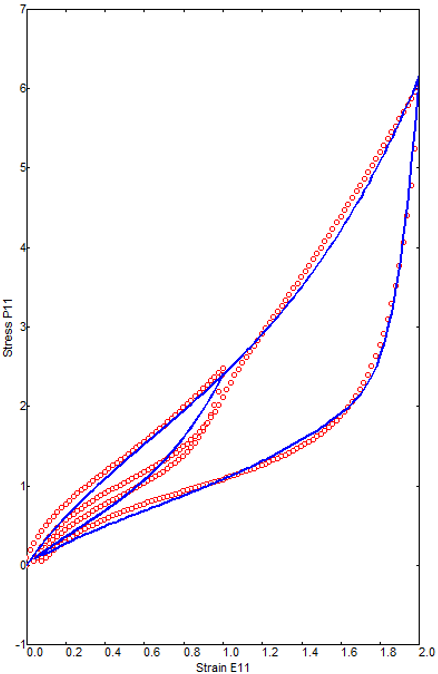
\includegraphics[height=6cm]{aproximace-ogden-roxburgh}
	\caption{Aproximace experimentu modelem Ogden-Roxburgh}
	\label{fig:aproximace-ogden-roxburgh}
\end{figure}
